\documentclass[conference]{IEEEtran}
\IEEEoverridecommandlockouts
% The preceding line is only needed to identify funding in the first footnote. If that is unneeded, please comment it out.
\usepackage{cite}
\usepackage{amsmath,amssymb,amsfonts}
\usepackage{algorithmic}
\usepackage{graphicx}
\usepackage{textcomp}
\def\BibTeX{{\rm B\kern-.05em{\sc i\kern-.025em b}\kern-.08em
    T\kern-.1667em\lower.7ex\hbox{E}\kern-.125emX}}
\begin{document}

\title{An Investigation into Search over Outsourced Encrypted Data}

\author{\IEEEauthorblockN{Student A}
\IEEEauthorblockA{Dept. of Computer Science \\
ID:12341000}
\and

\IEEEauthorblockN{Student B}
\IEEEauthorblockA{Dept. of Computer Science \\
ID:12341000}
\and

\IEEEauthorblockN{Student C}
\IEEEauthorblockA{Dept. of Computer Science \\
ID:12341000}
}

\maketitle


\section{Introduction}
Guidelines: In this section, you should abstract your target problem and present your motivation.
For example, you may highlight the practical motivation for encrypted search from your literature search. 
%
Meanwhile, you may categorize the typical research directions in the field of encrypted search (e.g., dynamic encrypted search, boolean encrypted search, and encrypted ranked search).
%
Further, you may present any particular security/practicality considerations on designing an encrypted search scheme.




If you want to use existing paper’s observations, please cite it like “In Song et al.'s work \cite{SongWP00}, the notion of searchable encryption is introduced for the first time.”



You can use figures/tables for illustration of your findings/ideas throughout the report. Table 1 and Fig. 1 are provided as examples.




\section{Application Setting}

\subsection{System Architecture}
Guidelines: In this subsection, you should describe the general application setting of encrypted search, e.g., how many parties are there in the real application setting, the particular role of each party, and the participation of each party (i.e., what each party does in  the work flow).

\subsection{Threat Model}

Guidelines: In this subsection, you should explain the threat assumptions generally adopted by the literature on encrypted search. For example, you may clearly indicate the trust assumptions of each party involved in the application (i.e., who is trusted or untrusted?), the goal of the untrusted party (e.g., what does the adversary want to learn?), how the adversary will behave, in a semi-honest fashion or in a malicious manner?


\begin{table}[h]
\centering
\caption{Comparison of encrypted search schemes.}
\label{my-label}
\begin{tabular}{|l|l|l|}
\hline
Scheme & Search Complexity & Index Size \\ \hline
\cite{SongWP00}   & ...              & ...       \\ \hline
...    & ...               & ...        \\ \hline
\end{tabular}
\end{table}


\section{Research Directions of Encrypted Search}
%

Guidelines: In this subsection, you should introduce the typical research directions for encrypted search, describe in detail the goals of each research direction in terms of functionality and/or security. You should also specify and discuss the design challenges in each direction based on your literature study and or your personal perspectives. Besides, you should properly discuss the existing works and try to reflect the state-of-the-art. A possible organization structure is given below. 


\begin{figure}[!t]
  \centering
  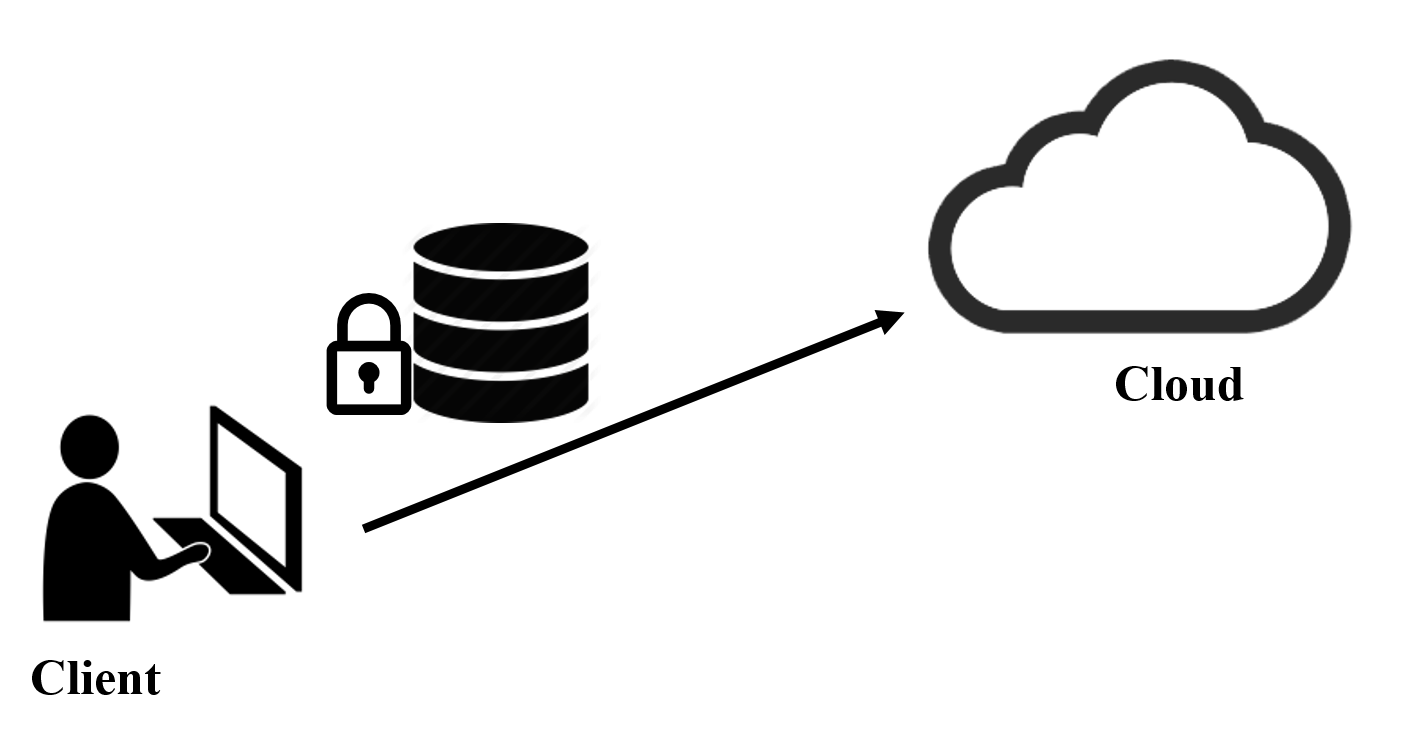
\includegraphics[width=2in]{./fig1.png}
  \caption{Outsourcing encrypted data to the cloud.}
  \label{fig_model}
\end{figure}

\subsection{Basic Searchable Encryption}

\textbf{Goals.} The description goes here.


\textbf{Design challenges.} The description goes here.

\textbf{Related work.} The description goes here.

\subsection{Dynamic Searchable Encryption}

\textbf{Goals.} The description goes here.


\textbf{Design challenges.} The description goes here.

\textbf{Related work.} The description goes here.




\subsection{Boolean Searchable Encryption}

\textbf{Goals.} The description goes here.


\textbf{Design challenges.} The description goes here.

\textbf{Related work.} The description goes here.

\subsection{Any Other Possible Categories}

\textbf{Goals.} The description goes here.


\textbf{Design challenges.} The description goes here.

\textbf{Related work.} The description goes here.

\section{Conclusion}

The conclusion goes here.


\bibliographystyle{IEEEtran}
\bibliography{references}


\end{document}
